\chapter{State of the Art}
\label{ch:sota}
	Over the years the research community has introduced various neural models for text classification.\autocites{Yang.2016}{Cho.2014}{Lee.2016}{Hochreiter.1997}{Kant.2018}{Zhou.2016}{Wang.2016}{Liang.2019}{Kim.2014}{Gao.2018}{Zhang.2015}{Johnson.2017}{Hoa.2017}{Yang.2018}{Rezaeinia.2018}{Zhao.2018}{Lai.2015}{Zheng.2019}{Johnson.2016}{Vaswani.2017}{Wang.2018b}{Iyyer.2015} In order to capture the whole variety of neural text classification models leaderboards, journals and academic full text databases have been screened for papers on neural text classification, namely:
	\begin{itemize}
		\item Association for Computational Linguistics \footnote{\url{https://www.aclweb.org/portal/}}
		\item Institute of Electrical and Electronics Engineers Xplore \footnote{\url{https://ieeexplore.ieee.org/Xplore/home.jsp}}
		\item Association for Computing Machinery Digital Library \footnote{\url{https://dl.acm.org/}}
		\item arXiv\footnote{\url{https://arxiv.org/}}
		\item Journal of Machine Learning Research\footnote{\url{http://www.jmlr.org/}}
		\item MIT Press Journals\footnote{\url{http://proceedings.mlr.press/}}
		\item Proceedings of Machine Learning Research\footnote{\url{http://proceedings.mlr.press/}}
		\item Papers With Code\footnote{\url{https://paperswithcode.com/}}
		\item GLUE\footnote{\url{https://gluebenchmark.com/leaderboard/}}
		\item NLP-Progress\footnote{\url{https://nlpprogress.com/}}
		\item Open AI\footnote{\url{https://openai.com/}}
		\item Google Scholar \footnote{\url{https://scholar.google.de/}}
	\end{itemize}
	The papers have been queried from these databases based on search queries created from Term Table \ref{tab:term_table} and selected based on the selection criteria listed in Section \ref{sec:selection_criteria}. Due to time constraints, this paper leaves out some databases, like Open Review\footnote{\url{https://openreview.net/}}. Nevertheless, this paper has analyzed over 100 papers on neural text classification. On that account, it is very likely all frequently used models are captured. The most used models are listed in Concept Matrix \ref{tab:concept_matrix} and described in this chapter. The concept matrix maps literature to the models they support. The remaining models are listed in Section \ref{sec:misc}.

	\section{\ac{CNN}}
		A highly regarded \ac{CNN} is the LeNet5 by Yann LeCun. LeNet5 was originally used for image classification. A grayscale image can be represented as matrix with each element corresponding to the grayscale of a pixel. Colored images can be represented in the same way by three matrices one for the red, green and blue scale value of a pixel. These matrices are called channels. A \ac{CNN} is structured like a \ac{MLP}, which neurons only connect partially to the input, see Figure \ref{img:cnn:neuron}. \autocite{LeCun.1998}
		\begin{figure}[H]
			\centering
			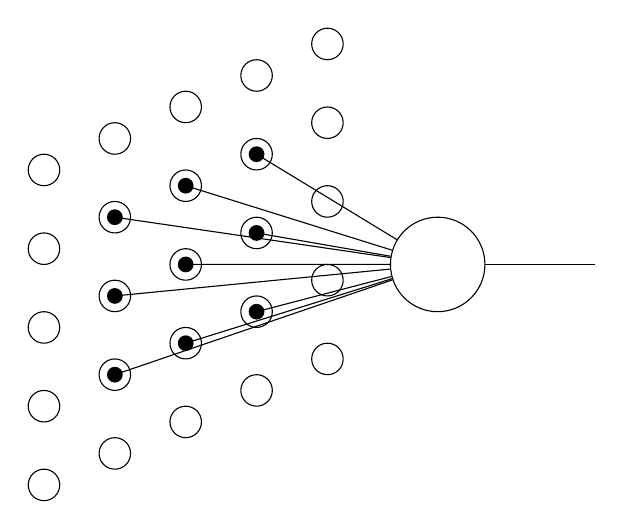
\begin{tikzpicture}
				\node[draw, circle, minimum size=1.2cm] (n) at (5,2.8) {};
				\draw (n) --  (7,2.8);
				\foreach \x in {0,1,2,3,4}
					\foreach \y in {0,1,2,3,4}
						\draw (\x*0.9+ \y*0, \x*0.4+\y*1) circle (0.2cm); %Matrixtransformation (0.7 0; 0.3 1)
				\foreach \x in {1,2,3}
					\foreach \y in {1,2,3} {
						\draw (\x*0.9+ \y*0, \x*0.4+\y*1) -- (n);
						\fill (\x*0.9+ \y*0, \x*0.4+\y*1) circle (0.1cm);
					}
			\end{tikzpicture}
			\caption{Neuron of a \ac{CNN} (own figure)} \label{img:cnn:neuron}
		\end{figure}
		In order to understand a \ac{CNN} three main operations need to be explained:
		\begin{itemize}
			\item Convolution
			\item Non Linearity
			\item Sub-Sampling
		\end{itemize}
		\paragraph{Convolution} in regard to \ac{CNN}s loosely refers to discrete convolution. Let the input matrix be $X$. Further, let the weight matrix of the \ac{CNN}'s neuron be $w$ with $k$ rows and $l$ columns called filter or kernel. Further, let the sub matrix resulting from the area the neuron is connected to be $X[i:i+l-1, j:j+k-1]$. Then the convolution is defined as \eqref{eq:convolution}.
			\begin{equation}
				\label{eq:convolution}
				X * w := w \cdot X[i:i+l-1, j:j+k-1] = O
			\end{equation}
		Meaning that each element of the resulting output matrix $O$ is the matrix product between the sub matrix of the area the neuron is connected to and the weight matrix of the neuron. The factor by which $i$ and $j$ are incremented determines the area the neuron is connected to. This factor is called $stride$. In consequence, an output matrix is produced for each kernel. The resulting output matrices are called activation maps or feature maps. \autocite{Zhang.2015c}
		\par
		In order to illustrate this abstract definition, consider the case of a grayscale image represented as a matrix $X$, as shown in Figure \ref{img:conv}. Furthermore, consider the kernel $w$, as shown in Figure \ref{img:conv}. Then, the convolution of the image and the kernel can be computed by laying the kernel on top of the image. The element of the activation map is computed by multiplying and summing the overlapping elements. To iterate through the elements the kernel is \enquote{slid} over each row and each column. Resulting in the output $O$, as shown in Figure \ref{img:conv}.
		\begin{figure}[H]
			\centering
			\begin{tikzpicture}
			\matrix (mtr) [matrix of nodes,row sep=-\pgflinewidth, nodes={draw}]
			{
				0 & 1 & 0 & |[fill=orange!30]| 1 & |[fill=orange!30]| 0 & |[fill=orange!30]| 0 & 0 & 0 & 0\\
				0 & 0 & 1 & |[fill=orange!30]| 1 & |[fill=orange!30]| 1 & |[fill=orange!30]| 0 & 0 & 1 & 0\\
				1 & 0 & 0 & |[fill=orange!30]| 1 & |[fill=orange!30]| 1 & |[fill=orange!30]| 1 & 0 & 1 & 0\\
				0 & 0 & 0 & 0 & 1 & 0 & 0 & 0 & 0\\
				0 & 0 & 1 & 1 & 0 & 1 & 0 & 0 & 1\\
				0 & 1 & 1 & 1 & 0 & 1 & 1 & 0 & 1\\
				0 & 1 & 1 & 0 & 0 & 0 & 1 & 1 & 0\\
			};
			
			\draw[very thick, orange] (mtr-1-4.north west) rectangle (mtr-3-6.south east);
			
			\node [below= of mtr-5-5.south] (lm) {$X$};
			
			\node[right = 0.2em of mtr] (str) {$\cdot$};
			
			\matrix (K) [right=0.2em of str,matrix of nodes,row sep=-\pgflinewidth, nodes={draw, fill=blue!30}]
			{
				1 & 0 & 1 \\
				0 & 1 & 0 \\
				1 & 0 & 1 \\
			};
			\node [below = of K-3-2.south] (lk) {$K$};
			
			\node [right = 0.2em of K] (eq) {$=$};
			
			\matrix (ret) [right=0.2em of eq,matrix of nodes,row sep=-\pgflinewidth, nodes={draw}]
			{
				1 & 4 & 2 & |[fill=black!30!green!30]| 4 & 1 & 2 & 1\\
				1 & 1 & 4 & 2 & 3 & 1 & 1\\
				2 & 2 & 2 & 5 & 1 & 3 & 1\\
				1 & 3 & 3 & 2 & 3 & 1 & 2\\
				3 & 3 & 2 & 2 & 2 & 3 & 2\\
			};
			\node [below = of ret-4-4.south] (lim) {$Y = \varphi(\sum X[i:i+k, j:j+k] \cdot K$};
			
			\draw[very thick, black!30!green] (ret-1-4.north west) rectangle (ret-1-4.south east);
			
			\draw[densely dotted, blue, thick] (mtr-1-4.north west) -- (K-1-1.north west);
			\draw[densely dotted, blue, thick] (mtr-3-4.south west) -- (K-3-1.south west);
			\draw[densely dotted, blue, thick] (mtr-1-6.north east) -- (K-1-3.north east);
			\draw[densely dotted, blue, thick] (mtr-3-6.south east) -- (K-3-3.south east);
			
			\draw[densely dotted, black!30!green, thick] (ret-1-4.north west) -- (K-1-1.north west);
			\draw[densely dotted, black!30!green, thick] (ret-1-4.south west) -- (K-3-1.south west);
			\draw[densely dotted, black!30!green, thick] (ret-1-4.north east) -- (K-1-3.north east);
			\draw[densely dotted, black!30!green, thick] (ret-1-4.south east) -- (K-3-3.south east);
			
			\matrix (K) [right=0.2em of str,matrix of nodes,row sep=-\pgflinewidth, nodes={draw, fill=blue!10}]
			{
				1 & 0 & 1 \\
				0 & 1 & 0 \\
				1 & 0 & 1 \\
			};
			
			\draw[very thick, blue] (K-1-1.north west) rectangle (K-3-3.south east);
			
			\node[anchor=south east, inner sep=0.01em, blue] at (mtr-1-4.south east) (xx) {\scalebox{.5}{$\times 1$}};
			\node[anchor=south east, inner sep=0.01em, blue] at (mtr-1-5.south east) (xx) {\scalebox{.5}{$\times 0$}};
			\node[anchor=south east, inner sep=0.01em, blue] at (mtr-1-6.south east) (xx) {\scalebox{.5}{$\times 1$}};
			\node[anchor=south east, inner sep=0.01em, blue] at (mtr-2-4.south east) (xx) {\scalebox{.5}{$\times 0$}};
			\node[anchor=south east, inner sep=0.01em, blue] at (mtr-2-5.south east) (xx) {\scalebox{.5}{$\times 1$}};
			\node[anchor=south east, inner sep=0.01em, blue] at (mtr-2-6.south east) (xx) {\scalebox{.5}{$\times 0$}};
			\node[anchor=south east, inner sep=0.01em, blue] at (mtr-3-4.south east) (xx) {\scalebox{.5}{$\times 1$}};
			\node[anchor=south east, inner sep=0.01em, blue] at (mtr-3-5.south east) (xx) {\scalebox{.5}{$\times 0$}};
			\node[anchor=south east, inner sep=0.01em, blue] at (mtr-3-6.south east) (xx) {\scalebox{.5}{$\times 1$}};
			
			\end{tikzpicture}
			\caption{Convolution Illustration (own figure)} \label{img:conv}
		\end{figure}
		As shown in Figure \ref{img:conv}, the resulting output is smaller than the original input. To preserve the original size, $padding$ may be used. $Padding$ can be described as adding zeros at the edges of the input. Therefore, the output size results in Equation \eqref{eq:conv:output}.\autocite{Conneau.2016}
		\begin{equation}
			output size = \frac{input size - kernel size + 2 \cdot padding}{stride} + 1
			\label{eq:conv:output}
		\end{equation}
		\paragraph{Non linearity} needs to be applied to the convolution in order to model non linearly correlated data, because the convolution as defined in \eqref{eq:convolution} is completely linear. Applying a non linear activation function $\varphi$ and a bias $b$ results in Equation \eqref{eq:conv:neuron}.\autocite{LeCun.1998}
		\begin{equation}
			y = \varphi(X * w + b) = \varphi(w \cdot X[i:i+l-1, j:j+k-1] + b)
			\label{eq:conv:neuron}
		\end{equation}
		Thus, Equation \eqref{eq:conv:neuron} is rather similar to Equation \eqref{eq:neuron:y} which is used in Section \ref{sec:neuron} to describe a neuron. The only difference is the shape of the input the neuron is connected to. Deducing from this, neurons of a \ac{MLP} and a \ac{CNN} do not differ in their structure.
		\paragraph{Sub-sampling} is used after convolution and non linearity are applied. \autocite{LeCun.1998} Sub-sampling means reducing the size of the feature maps. The computational complexity of a \ac{CNN} increases over depth in regard to the number and size of the feature maps.\autocites{Conneau.2016}{Johnson.2017} Due to that, sub-sampling reduces the computational complexity in multi layer \ac{CNN}s. Sub-sampling can be achieved by different strategies. However, \cite{Zhang.2015c} found that max pooling outperforms other sub-sampling strategies. Max pooling is defined as \eqref{eq:maxp}.\autocite{Boureau.2010}
		\begin{equation}
			\label{eq:maxp}
			MaxPooling(X) := max(X[i:i+l-1, j:j+k-1])
		\end{equation}
		Accordingly, max pooling works similar to convolution. The pooling kernel is \enquote{slid} over the input matrix, but instead of convolving the sub matrix and the filter, the maximum of the sub matrix is taken, see Figure \ref{img:maxp}.
		\begin{figure}[H]
			\centering
			\begin{tikzpicture}
			\matrix (mtr) [matrix of nodes,row sep=-\pgflinewidth, nodes={draw}]
			{
				0 & 1 & 0 & |[fill=orange!30]| 1 & |[fill=orange!30]| 0 & |[fill=orange!30]| 0 & 0 & 0 & 0\\
				0 & 0 & 4 & |[fill=orange!30]| 1 & |[fill=orange!30]| 2 & |[fill=orange!30]| 0 & 0 & 1 & 0\\
				2 & 0 & 0 & |[fill=orange!30]| 1 & |[fill=orange!30]| 4 & |[fill=orange!30]| 1 & 0 & 1 & 0\\
				0 & 0 & 0 & 0 & 1 & 0 & 3 & 0 & 0\\
				0 & 0 & 1 & 1 & 0 & 1 & 0 & 0 & 0\\
				0 & 1 & 1 & 3 & 0 & 1 & 0 & 0 & 0\\
				0 & 1 & 1 & 0 & 0 & 0 & 1 & 1 & 0\\
			};
			
			\draw[very thick, orange] (mtr-1-4.north west) rectangle (mtr-3-6.south east);
			
			\node [below= of mtr-5-5.south] (lm) {$\bf X$};
			
			\node [below = of K-3-2.south] (lk) {$\bf Kernel$};
			
			\matrix (ret) [right=0.2em of eq,matrix of nodes,row sep=-\pgflinewidth, nodes={draw}]
			{
				4 & 4 & 4 & |[fill=black!30!green!30]| 4 & 4 & 1 & 1\\
				4 & 4 & 4 & 4 & 4 & 3 & 3\\
				2 & 1 & 4 & 4 & 4 & 3 & 3\\
				1 & 3 & 3 & 3 & 3 & 3 & 3\\
				1 & 3 & 3 & 3 & 1 & 1 & 1\\
			};
			\node [below = of ret-4-4.south] (lim) {${\bf MaxPooling(X)}$};
			
			\draw[very thick, black!30!green] (ret-1-4.north west) rectangle (ret-1-4.south east);
			
			\draw[densely dotted, blue, thick] (mtr-1-4.north west) -- (K-1-1.north west);
			\draw[densely dotted, blue, thick] (mtr-3-4.south west) -- (K-3-1.south west);
			\draw[densely dotted, blue, thick] (mtr-1-6.north east) -- (K-1-3.north east);
			\draw[densely dotted, blue, thick] (mtr-3-6.south east) -- (K-3-3.south east);
			
			\draw[densely dotted, black!30!green, thick] (ret-1-4.north west) -- (K-1-1.north west);
			\draw[densely dotted, black!30!green, thick] (ret-1-4.south west) -- (K-3-1.south west);
			\draw[densely dotted, black!30!green, thick] (ret-1-4.north east) -- (K-1-3.north east);
			\draw[densely dotted, black!30!green, thick] (ret-1-4.south east) -- (K-3-3.south east);
			
			\matrix (K) [right=0.2em of str,matrix of nodes,row sep=-\pgflinewidth, nodes={draw, fill=blue!10}]
			{
				 &  & \\
				 &  & \\
				 &  & \\
			};
			
			\draw[very thick, blue] (K-1-1.north west) rectangle (K-3-3.south east);
			
			\end{tikzpicture}
			\caption{Max Pooling Illustration (own figure)} \label{img:maxp}
		\end{figure}
		\par
		These three operations form the basic building block of a \ac{CNN}. This building block is comprised of a convolutional layer followed by a non linearity. The pooling layer is applied after the non linearity and is optional. This building block can be repeated any number of times. \autocite{LeCun.1998} This is illustrated in Figure \ref{img:cnn}.
		\begin{figure}[H]
			\centering
			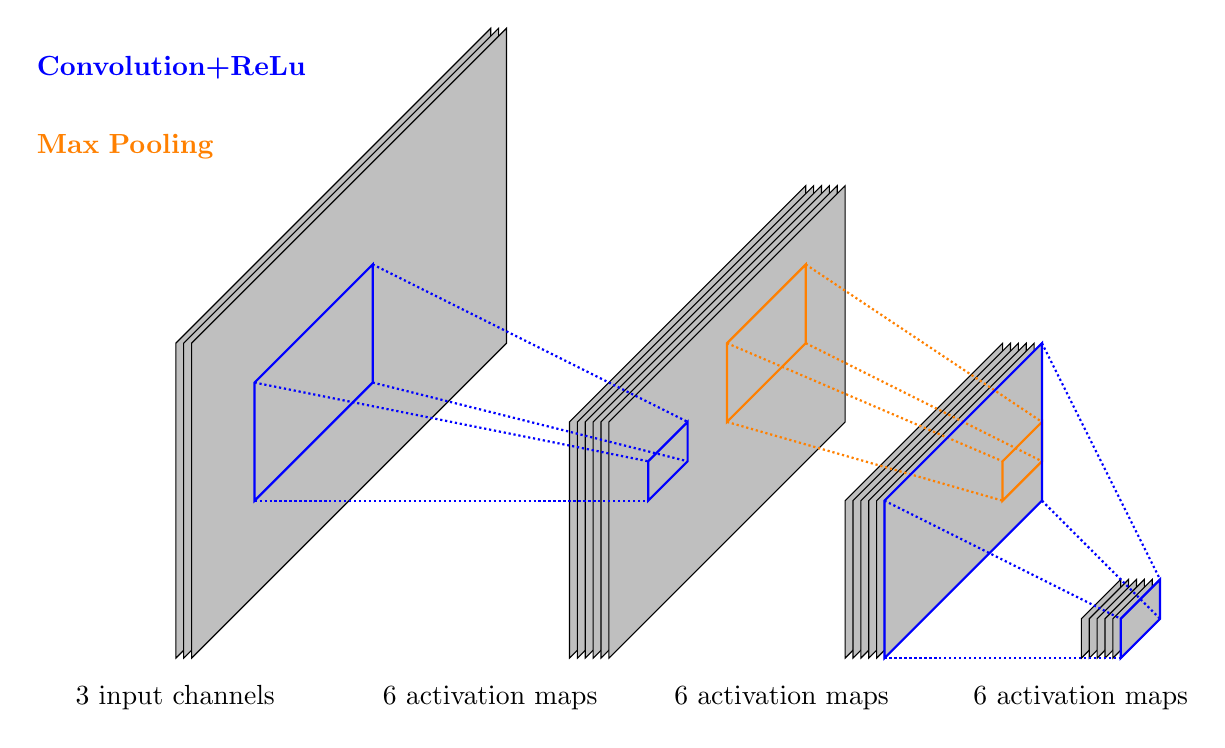
\begin{tikzpicture}
	\begin{scope}[yslant=1,xshift=0.2]
		\foreach \i in {0,0.1,0.2}
			\draw [fill=lightgray] (0+\i,0-\i) rectangle (4+\i,4-\i);
		
		\foreach \i in {0,0.1,0.2,0.3,0.4,0.5}
			\draw [fill=lightgray] (5+\i,-5-\i) rectangle (8+\i,-2-\i);
			
		\foreach \i in {0,0.1,0.2,0.3,0.4,0.5}
			\draw [fill=lightgray] (8.5+\i,-8.5-\i) rectangle (10.5+\i,-6.5-\i);
			
		\foreach \i in {0,0.1,0.2,0.3,0.4,0.5}
			\draw [fill=lightgray] (11.5+\i,-11.5-\i) rectangle (12+\i,-11-\i);
		
		\draw [thick, blue] (1,1) rectangle (2.5,2.5);
		\draw [thick, blue] (6,-4) rectangle (6.5,-3.5);
		\draw[densely dotted, blue, thick] (1,1) -- (6,-4);
		\draw[densely dotted, blue, thick] (1,2.5) -- (6,-3.5);
		\draw[densely dotted, blue, thick] (2.5,1) -- (6.5,-4);
		\draw[densely dotted, blue, thick] (2.5,2.5) -- (6.5,-3.5);
		
		\draw [thick, orange] (7,-4) rectangle (8,-3);
		\draw [thick, orange] (10.5,-8) rectangle (11,-8.5);
		\draw[densely dotted, orange, thick] (7,-4) -- (10.5,-8.5);
		\draw[densely dotted, orange, thick] (7,-3) -- (10.5,-8);
		\draw[densely dotted, orange, thick] (8,-4) -- (11,-8.5);
		\draw[densely dotted, orange, thick] (8,-3) -- (11,-8);
		
		\draw [thick, blue] (9,-9) rectangle (11,-7);
		\draw [thick, blue] (12,-12) rectangle (12.5,-11.5);
		\draw[densely dotted, blue, thick] (9,-9) -- (12,-12);
		\draw[densely dotted, blue, thick] (9,-7) -- (12,-11.5);
		\draw[densely dotted, blue, thick] (11,-9) -- (12.5,-12);
		\draw[densely dotted, blue, thick] (11,-7) -- (12.5,-11.5);
	\end{scope}
	
	\node (in) at (0,-0.5) {3 input channels};
	\node (h1) at (4,-0.5) {6 activation maps};
	\node (h2) at (7.7,-0.5) {6 activation maps};
	\node (out) at (11.5,-0.5) {6 activation maps};
	
	\node [text=blue, align=left,text width=10em] (conv) at (0,7.5) {\bf Convolution+ReLu};
	\node [text=orange, align=left,text width=10em] (pool) at (0,6.5) {\bf Max Pooling};
\end{tikzpicture}
			\caption{\ac{CNN} (own figure)} \label{img:cnn}
		\end{figure}
	\paragraph{For text classification} the \ac{CNN} works in the same way. The input for text classification can be described as a sequence of words. These words can be embedded as vectors which are concatenated into a sequence matrix. This sequence matrix is the input channel to the \ac{CNN}.\autocite{Kim.2014}
		
	\section{\ac{RNN}}
		A \ac{RNN} is structured like a \ac{MLP} with neurons connect to themselves, see Figure \ref{img:rnn}. \autocite{Elman.1990} Due to that, the output of a \ac{RNN}, in contrast to a \ac{MLP}, is dependent on previous computations. On this account, \ac{RNN}s are able to process sequential information like text. A text can be seen as a sequence of words. These words can be encoded as vectors. \autocites{Wang.2012}{Turian.2010}{Mikolov.2013}{Mikolov.2013b}{Joulin.2016}{Smith.2019}{Pennington.2014}{McCann.2017} This results in a sequence of vectors. Each element of that sequence is processed in the same way. That is why \ac{RNN}s are called recurrent. 
		\begin{figure}[H]
			\centering
			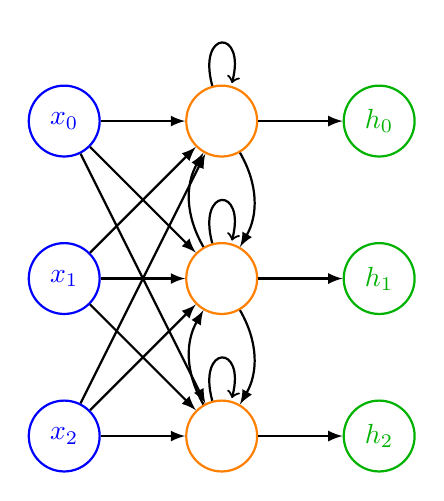
\begin{tikzpicture}[-latex,auto,node distance=2cm,thick]
	
	\node [draw, circle, minimum size=0.9cm,blue] (A) at (0,0) {$x_0$};
	\node [draw, circle, minimum size=0.9cm,orange] (B) [right of=A] {};
	\node [draw, circle, minimum size=0.9cm,black!30!green] (C) [right of=B] {$h_0$};
	
	\node [draw, circle, minimum size=0.9cm,blue] (D) [below of=A] {$x_1$};
	\node [draw, circle, minimum size=0.9cm,orange] (E) [right of=D] {};
	\node [draw, circle, minimum size=0.9cm,black!30!green] (F) [right of=E] {$h_1$};
	
	\node [draw, circle, minimum size=0.9cm,blue] (G) [below of=D] {$x_2$};
	\node [draw, circle, minimum size=0.9cm,orange] (H) [right of=G] {};
	\node [draw, circle, minimum size=0.9cm,black!30!green] (I) [right of=H] {$h_2$};
	
	\path (A) edge (B) (B)	edge (C) (B) edge [loop above] (B)
		(D) edge (E) (E)	edge (F) (E) edge [loop above] (E)
		(G) edge (H) (H)	edge (I) (H) edge [loop above] (H)
		(B) edge [bend left] (E) (E)	edge [bend left] (H)
		(H) edge [bend left] (E) (E)	edge [bend left] (B)
		(A) edge (E) (A) edge (H) (D) edge (B) (D) edge (H) (G) edge (B) (G) edge (E);
\end{tikzpicture}
			\caption{Recurrent Neural Network (own figure)} \label{img:rnn}
		\end{figure}
		As shown in Section \ref{sec:mlp}, connections can be described using a weight matrix. Therefore, let the recurrent connections be described by the weight matrix $W^{(hh)}$ and the connections to the input by the weight matrix $W^{(hx)}$. Further let the input vector $x_t$ be element of the  sequence $(x_1, x_2 \dots x_n)$. Then the information, carried between each time step $t$ of the sequence, called hidden state $h_t$, can be described as \eqref{eq:rnn:hiddenstate}.
		\begin{equation}
			h_t = \varphi(W^{(hh)}h_{t-1}+W^{(hx)}x_t)
			\label{eq:rnn:hiddenstate}
		\end{equation}
		Consequently, in theory \ac{RNN}s are able to propagate information through arbitrarily long sequences. However, in practice they are limited to only a few time steps. This is because of the vanishing gradient problem. \autocite{Hochreiter.2001} In order to overcome the vanishing gradient problem \ac{LSTM} \autocite{Hochreiter.1997} and \ac{GRU} \autocite{Cho.2014} were designed. Both variations use gated units and a memory vector to directly propagate information between time steps, thus preventing the information from vanishing. \autocite{Hochreiter.2001} According to the results of the papers reviewed for the Concept Matrix \ref{tab:concept_matrix}, both variations perform much better than vanilla \ac{RNN}s. However, neither \ac{GRU}s, nor \ac{LSTM}s seem to have a significant performance advantage over the other.\autocites{Greff.2015}{Shah.2015} As more of the reviewed papers used \ac{LSTM}s, this paper only introduces \ac{LSTM}s. A \ac{LSTM} consists of one \ac{LSTM} cell per time step in a sequence.
		A \ac{LSTM} cell at time step $t$ consists of an input gate $i_t$, an output gate $o_t$, a forget gate $f_t$ and a cell state $c_t$, see Figure \ref{img:lstm}. The cell state runs along the entire sequence only influenced by information filtered through the input and forget gate. Therefore, information can be preserved over a long sequence.
		Gates use the sigmoid function $\sigma$ and element wise multiplication $\otimes$ to block or convey information. The sigmoid function \enquote{squashes} all values in the range of $[0;1]$,  thus creating a vector which scalars are in the range of $[0;1]$. Any scalar multiplied by $0$ is $0$. Due to that, any information conveyed by that scalar is blocked. Accordingly, any multiplier above $0$ conveys a portion of the information. In consequence, the element wise multiplication multiplies all scalars with a scalar in range of $[0;1]$.
		The forget gate applies this operations to the cell state. The scalars of the cell state multiplied by $0$ are \enquote{forgotten}. The input gate applies a non linearity to the input information, and uses the gating mechanism to decide what part of that information is added to the cell state. The resulting information is called new cell content $\tilde{c_t}$. The output gate applies a non linearity to the cell state, and uses the information conveyed by the input gate for its own gating mechanism to decide what information of the cell state is returned as output. The output is called hidden state $h_t$.
		\begin{figure}[H]
			\centering
			% Code mostly compypasted from By J. Leon, Beerware licence is acceptable..., under https://tex.stackexchange.com/questions/432312/how-do-i-draw-an-lstm-cell-in-tikz

\begin{tikzpicture}[
	% GLOBAL CFG
	font=\sf \scriptsize,
	>=LaTeX,
	% Styles
	cell/.style={% For the main box
		rectangle, 
		rounded corners=5mm, 
		draw,
		very thick,
	},
	operator/.style={%For operators like +  and  x
		circle,
		draw,
		inner sep=-0.5pt,
		minimum height =.2cm,
	},
	function/.style={%For functions
		ellipse,
		draw,
		inner sep=1pt
	},
	ct/.style={% For external inputs and outputs
		circle,
		draw,
		line width = .75pt,
		minimum width=1cm,
		inner sep=1pt,
	},
	gt/.style={% For internal inputs
		rectangle,
		draw,
		minimum width=4mm,
		minimum height=3mm,
		inner sep=1pt
	},
	mylabel/.style={% something new that I have learned
		font=\scriptsize\sffamily, 
		align=center,
	},
	ArrowC1/.style={% Arrows with rounded corners
		rounded corners=.25cm,
		thick,
	},
	ArrowC2/.style={% Arrows with big rounded corners
		rounded corners=.5cm,
		thick,
	},
	]
	
	%Start drawing the thing...  
	\draw[orange, fill=orange!30,rounded corners=5mm] (-3,-2) rectangle (-1.77,2);
	\draw[blue, fill=blue!30,rounded corners=5mm] (-1.75,-2) rectangle (0.18,1);
	\draw[black!30!green, fill=black!30!green!30,rounded corners=5mm] (0.2,-2) rectangle (2.25,1.25);
	\node[orange] (f) at (-5,0) {\bf \large forget gate};
	\node[blue] (i) at (0,-3) {\bf \large input gate};
	\node[black!30!green] (o) at (5,0) {\bf \large output gate};
	% Draw the cell: 
	\node [cell, minimum height =4cm, minimum width=6cm] at (0,0){} ;
	
	% Draw inputs named ibox#
	\node [gt] (ibox1) at (-2,-0.75) {$\sigma$};
	\node [gt] (ibox2) at (-1.5,-0.75) {$\sigma$};
	\node [gt, minimum width=1cm] (ibox3) at (-0.5,-0.75) {Tanh};
	\node [gt] (ibox4) at (0.5,-0.75) {$\sigma$};
	
	% Draw opérators   named mux# , add# and func#
	\node [operator] (mux1) at (-2,1.5) {$\times$};
	\node [operator] (add1) at (-0.5,1.5) {+};
	\node [operator] (mux2) at (-0.5,0) {$\times$};
	\node [operator] (mux3) at (1.5,0) {$\times$};
	\node [function] (func1) at (1.5,0.75) {Tanh};
	
	% Draw External inputs? named as basis c,h,x
	\node[ct, label={[mylabel]Previous \\ Cell State}] (c) at (-4,1.5) {$c_{t-1}$};
	\node[ct, label={[mylabel]Previous \\ Hidden State}] (h) at (-4,-1.5) {$h_{t-1}$};
	\node[ct, label={[mylabel]left:Input}] (x) at (-2.5,-3) {$x_t$};
	
	% Draw External outputs? named as basis c2,h2,x2
	\node[ct, label={[mylabel]Cell State}] (c2) at (4,1.5) {$c_t$};
	\node[ct, label={[mylabel]Hidden State}] (h2) at (4,-1.5) {$h_t$};
	\node[ct, label={[mylabel]left:Hidden State}] (x2) at (2.5,3) {$h_t$};
	
	% Start connecting all.
	%Intersections and displacements are used. 
	% Drawing arrows    
	\draw [ArrowC1] (c) -- (mux1) -- (add1) -- (c2);
	\draw [ArrowC1] (c) -- (-2.5, 1.5) -- (-2.5, -1.5) -- (-2, -1.5) -- (ibox1);
	
	% Inputs
	\draw [ArrowC2] (h) -| (ibox4);
	\draw [ArrowC1] (h -| ibox1)++(-0.5,0) -| (ibox1); 
	\draw [ArrowC1] (h -| ibox2)++(-0.5,0) -| (ibox2);
	\draw [ArrowC1] (h -| ibox3)++(-0.5,0) -| (ibox3);
	\draw [ArrowC1] (x) -- (x |- h)-| (ibox3);
	
	% Internal
	\draw [-latex, ArrowC2] (ibox1) -- (mux1);
	\draw [-latex, ArrowC2] (ibox2) |- (mux2);
	\draw [-latex, ArrowC2] (ibox3) -- (mux2);
	\draw [-latex, ArrowC2] (ibox4) |- (mux3);
	\draw [-latex, ArrowC2] (mux2) -- (add1);
	\draw [-latex, ArrowC1] (add1 -| func1)++(-0.5,0) -| (func1);
	\draw [-latex, ArrowC2] (func1) -- (mux3);
	
	%Outputs
	\draw [-, ArrowC2] (mux3) |- (h2);
	\draw (c2 -| x2) ++(0,-0.1) coordinate (i1);
	\draw [-, ArrowC2] (h2 -| x2)++(-0.5,0) -| (i1);
	\draw [-, ArrowC2] (i1)++(0,0.2) -- (x2);

\end{tikzpicture}
			\caption{LSTM Cell (based on \cite{Graves.2013})} \label{img:lstm}
		\end{figure}
		As described so far, the gates do not know what information to block or convey. That is why \ac{MLP}s are used inside the gates, having either $Tanh$ or $\sigma$ as their activation function. These \ac{MLP}s learn to operate the gates. They consist of an input layer, an output layer and one hidden layer. As shown in Section \ref{sec:mlp}, these layers can be described by matrices, denoted $W$. In consequence, a \ac{LSTM} can be described as in Equation \eqref{eq:lstm}. \autocite{Graves.2013} 
		\footnote{As Figure \ref{img:lstm} shows a concatenation while Equation \eqref{eq:lstm} uses a sum operation, it is reasonable to point out that these are equal. $[x_t; h_{t-1}; c_{t-1}] \dot [W_x; W_h; W_c] = x_tW_h + h_{t-1}W_h + c_{t-1}tW_c$}
		\begin{equation}
			\label{eq:lstm}
			\begin{array}{lcl}
				i_t & = & \sigma(W_{xi}x_t + W_{hi}h_{t-1} + W_{ci}c_{t-1} + b_i) \\
				o_t & = & \sigma(W_{xo}x_t + W_{ho}h_{t-1} + W_{co}c_{t-1} + b_o) \\
				f_t & = & \sigma(W_{xf}x_t + W_{hf}h_{t-1} + W_{cf}c_{t-1} + b_f) \\
				\tilde{c_t} & = & Tanh(W_{xc}x_t + W_{hc}h_{t-1} + W_{cc}c_{t-1} + b_c) \\
				c_t & = & i_t \otimes \tilde{c_t} + f_t \otimes c_{t-1} \\
				h_t & = & o_t \otimes Tanh(c_t)
			\end{array}
		\end{equation}
		
	\section{Transformer}
	Architectures based on the Transformer namely BERT \autocite{Devlin.2018}, ALBERT \autocite{Lan.2019} and XLNet \autocite{Yang.2019} dominate the top of the GLUE leaderboard\autocite{Wang.2019}.  \footnote{\url{https://gluebenchmark.com/leaderboard/}} The Transformer, originally introduced by \cite{Vaswani.2017}, mainly utilizes a mechanism called attention. The Transformer is comprised of an encoder and a decoder. However, only the encoder or a modified version of the encoder is used by BERT, ALBERT and XLNet. For this reason, this section focuses on the Transformer encoder. 
	
	The encoder is composed of a stack of $N+1$ Blocks. The first block is comprised of an input embedding and a positional encoder. The remaining $N$ blocks are Transformer blocks. The input to the Transformer encoder is a sequence of words of length $T$. The output of each block is a sequence of hidden states $h_t^{(n)}$ where $t$ is the position in the sequence and $n$ is the block. $n=0$ denotes the first block. As a result, the input of each block is the sequence of previous hidden states. Each block is composed of two layers. The first is a multi-head self-attention mechanism, and the second is a \ac{MLP}. A residual connection\autocite{He.2015}, followed by layer normalization \autocite{Ba.2016} is employed around each of the two layers. Therefore, the output of each layer can be described as in Equation \eqref{eq:transformer}.
	\begin{equation}
		\label{eq:transformer}
		LayerNorm(x + Layer(x))
	\end{equation} 
	With $Layer(x)$ being the function of the layer itself and $LayerNorm(x)$ being the function described by \cite{He.2015}, the residual connections bypass the layers and allow the input to flow past them unchanged. On that account, a residual connection can be described as summing the input vectors to the output vectors. Hence, the inputs and outputs of all layers in the model need to be of the same dimensionality. The Transformer encoder is shown in Figure \ref{img:transformer}.
	\begin{figure}[H]
		\centering
		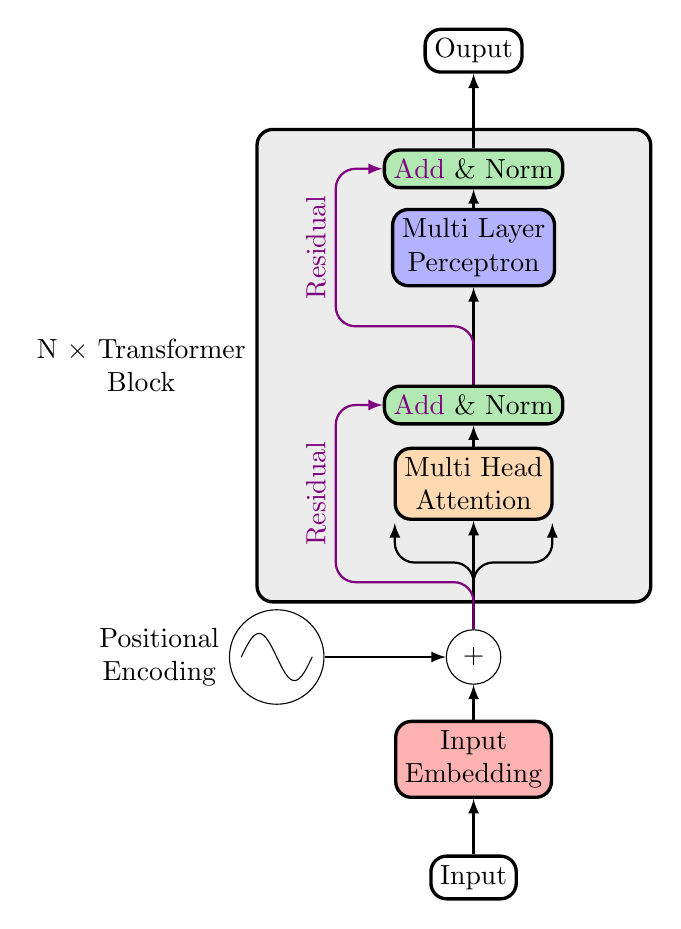
\begin{tikzpicture}[
	cell/.style={
		rectangle, 
		rounded corners=2mm, 
		draw,
		very thick,
		align=center,
	},
	ArrowC1/.style={% Arrows with rounded corners
		rounded corners=.25cm,
		thick,
	},
	do path picture/.style={%
		path picture={%
			\pgfpointdiff{\pgfpointanchor{path picture bounding box}{south west}}%
			{\pgfpointanchor{path picture bounding box}{north east}}%
			\pgfgetlastxy\x\y%
			\tikzset{x=\x/2,y=\y/2}%
			#1
		}
	},
	sin wave/.style={do path picture={    
			\draw [line cap=round] (-3/4,0)
			sin (-3/8,1/2) cos (0,0) sin (3/8,-1/2) cos (3/4,0);
	}},
]
	\node [cell] (out) at (0,10.5) {Ouput};
	
	\node [cell, fill=lightgray!30, minimum height=6cm, minimum width=5cm, label={[align=center]left:N $\times$ Transformer \\ Block}] (tb) at (-0.25,6.5) {};
	\node [cell, fill=black!30!green!30] (an2) at (0,9) {\textcolor{violet}{Add} \& Norm};
	\node [cell, fill=blue!30] (mlp) at (0,8) {Multi Layer \\ Perceptron};
	\node [cell, fill=black!30!green!30] (an1) at (0,6) {\textcolor{violet}{Add} \& Norm};
	\node [cell, fill=orange!30] (mha) at (0,5) {Multi Head \\ Attention};
	
	
	\node [draw, circle] (+) at (0,2.8) {$+$};
	\node [cell, fill=red!30] (emb) at (0,1.5) {Input \\ Embedding};
	\node [cell] (in) at (0,0) {Input};
	\node[circle, draw, sin wave, minimum size=1.2cm, label={[align=center]left:Positional \\ Encoding}] (pos) at (-2.5,2.8) {};
	
	\draw [-latex,ArrowC1] (in) -- (emb);
	\draw [-latex,ArrowC1] (emb) -- (+);
	\draw [-latex,ArrowC1] (+) -- (0,4) -- (mha);
	\draw [-latex,ArrowC1] (mha) -- (an1);
	\draw [-latex,ArrowC1] (an1) -- (0,7) -- (mlp);
	\draw [-latex,ArrowC1] (mlp) -- (an2);
	\draw [-latex,ArrowC1] (an2) -- (out);
	\draw [-latex, ArrowC1] (pos) -- (+);
	
	\draw [-latex, ArrowC1] (+) -- (0,4) -- (1,4) -- (1,4.5);
	\draw [-latex, ArrowC1] (+) -- (0,4) -- (-1,4) -- (-1,4.5);
	
	\draw [-latex, ArrowC1,violet] (+) -- (0,3.75) -- (-1.75, 3.75) -- (-1.75,3.5 |- an1) node[sloped,above,midway] {Residual} -- (an1);
	\draw [-latex, ArrowC1,violet] (an1) -- (0,7) -- (-1.75, 7) -- (-1.75,7 |- an2) node[sloped,above,midway] {Residual} -- (an2);
\end{tikzpicture}
		\caption{Transformer Encoder (based on \cite{Vaswani.2017})} \label{img:transformer}
	\end{figure}
	\paragraph{Multi-Head Attention} is described in the following paragraph.
	\blockcquote{Vaswani.2017}{An attention function can be described as mapping a query and a set of key-value pairs to an output, where the query, keys, values, and output are all vectors. The output is computed as a weighted sum of the values, where the weight assigned to each value is computed by a compatibility function of the query with the corresponding key.}
	\cite{Vaswani.2017} use dot-product attention \autocite{Bahdanau.2014} scaled by the dimension $d_k$ of the keys. To obtain the scaled dot-product attention the dot-product of the queries with all keys, each divided by $\sqrt{d_k}$ is computed. Subsequently, a softmax function is applied to obtain the weights on the values. At last the values are weighted. The input to a Transformer Block is the sequence of previous hidden states. These hidden states form the queries, the keys and the values. Resulting from this, queries, keys and values are the same, so the attention of a query is to the query itself. For this reason, this kind of attention is called self-attention. In practice, the attention function can be computed on all queries simultaneously, by concatenating the queries into a matrix $Q$, the keys into a matrix $K$ and the values into a matrix $V$, see Equation \eqref{eq:attention}. \autocite{Vaswani.2017}
	\begin{equation}
		\label{eq:attention}
		Attention(Q,K,V)=softmax(\frac{QK^{{\mathrm {T}}}}{\sqrt{d_k}})V
	\end{equation}
	\blockcquote{Vaswani.2017}{Multi-head attention allows the model to jointly attend to information from different representation subspaces at different positions. With a single attention head, averaging inhibits this.}
	Multi-head attention linearly projects the queries, keys and values $h$ times to $d_k$ dimensions. The projection matrices $W_i^Q$, $W_i^K$ and $W_i^V, i \in [1;h]$ are individually learned and thus differ from each other.
	The attention function is applied to each of these projections. The resulting matrices are concatenated and again projected. Resulting in a matrix, being the multi-head attentions output. This is shown in Equation \eqref{eq:multiheadattention}. \autocite{Vaswani.2017}
	\begin{equation}
		\label{eq:multiheadattention}
		\begin{array}{rcl}
			MultiHead(Q,K,V) & = & Concat(head_1, head_2, \dots head_h) W^O \\
			\text{where }head_i & = & Attention(QW_i^Q,KW_i^K,VW_i^V)
		\end{array}
	\end{equation}
	\paragraph{\ac{MLP}s} cannot be applied to matrices. This is a problem, because the multi-head attention, as described in Equation \eqref{eq:multiheadattention} returns a matrix. However, this matrix is comprised of attention vectors. On this account one \ac{MLP} can be applied per attention vector. \autocite{Vaswani.2017}
	\paragraph{Input embeddings} are used to convert tokens to vectors. The input embedding is a learned embedding. This is similar to other embedding approaches, like \cites{Wang.2012}{Turian.2010}{Mikolov.2013}{Mikolov.2013b}{Joulin.2016}{Smith.2019}{Pennington.2014}{McCann.2017}. \autocite{Vaswani.2017}
	\paragraph{Positional Encoding} is used to inject information about a token's relative or absolute position in the input sequence. This is necessary since the attention mechanism, unlike recurrence or convolution, does not preserve spatial information. In order to be summed, positional encoding and input embedding must have the same dimensionality $d$. Each embedded token is a vector of size $d$. Consequently the positional encoding must return a scalar for each dimension $i \in [1,d]$ \autocite{Vaswani.2017}. \cite{Vaswani.2017} uses the sine and cosine functions of different frequencies to encode a token's position $pos$ in the input sequence , as shown in Equation \eqref{eq:posemb}.
	\begin{equation}
		\label{eq:posemb}
		\begin{array}{rcl}
			PositionEmbedding(pos,2i) & = & sin(\frac{pos}{100000^{2 / d}}) \\
			PositionEmbedding(pos,2i+1) & = & cos(\frac{pos}{100000^{2 / d}})
		\end{array}
	\end{equation}
		
	\section{Miscellaneous}
	\label{sec:misc}
	 The remaining models found in the course of the literature review are listed below.
	 \begin{itemize}
	 	\item Deep Averaging Network
	 	\item Hierarchical Attention Network
	 	\item Capsule Network
	 	\item Hierarchical Ensemble
	 	\item CNN-RNN Ensemble
	 	\item RNN-CNN Ensemble
	 \end{itemize}
 	The Deep Averaging Network uses less training time per epoch, but this comes at the cost of weaker performance \autocites{Iyyer.2015}{Cer.2018},
 	the Hierarchical Attention Network is outperformed by a \ac{LSTM} \autocite{Adhikari.2019} and
 	the Capsule Network while shown to outperforming simple \ac{LSTM}s and \ac{CNN}s \autocites{Xiao.2018}{Kim.2018}{Srivastava.2018}{Ren.2018}{Zhao.2018}, does not surpass some designed \ac{LSTM}s and \ac{CNN}s on top of the GLUE\footnote{\url{https://gluebenchmark.com/leaderboard/}}, NLP Progress\footnote{\url{https://nlpprogress.com/english/text_classification.html}} and Papers With Code\footnote{\url{https://paperswithcode.com/task/text-classification}} leaderboards. For these reasons Deep Averaging Networks, Hierarchical Attention Networks and Capsule Networks are not further investigated in this paper.
 	\par
 	Ensembles in general are not single neural network architectures but an ensemble comprised of models. The Hierarchical Ensemble uses one model, for example a \ac{LSTM}, to encode word vectors into sentence vectors and the same or another model to encode the sentence vectors into a document vector. Subsequently a softmax classifier is applied to the document vector. The remaining ensembles use similar strategies. A RNN-CNN Ensemble encodes a sequence of vectors into a matrix using an \ac{LSTM}, then a \ac{CNN} is applied to that matrix. A CNN-RNN Ensemble encodes a matrix into a sequence of vectors using a \ac{CNN}. Subsequently this sequence is used as input to a \ac{LSTM}. These models are not explained separately as they simply consist of \ac{CNN}s and \ac{RNN}s. However, ensembles are considered for the proposed model.